\documentclass[a4j,11pt]{jarticle}
%\usepackage[dviout]{graphicx}
\usepackage[dvipdfmx]{graphicx}
\usepackage{amsmath}
\usepackage{amssymb}
\usepackage{ascmac}
%\usepackage{epsbox}
\usepackage{float}
\usepackage{here}
\usepackage{lscape}
\usepackage{latexsym}
\usepackage{pifont}
\usepackage{wrapfig}
\usepackage{type1cm}
\usepackage{algorithm}
\usepackage{algorithmic}
\usepackage{txfonts}
\usepackage{bm}
\usepackage{comment}
\usepackage{url}
%\usepackage{natbib}
%\usepackage[square]{natbib}

\usepackage{listings}
%\usepackage{plistings}

%\setlength{\voffset}{-25.4mm}
\setlength{\topmargin}{-17.5mm}   %トップとヘッダの間隔
%\setlength{\headheight}{20mm}   %ヘッダの高さ
%\setlength{\headsep}{0mm}   %ヘッダとテキストの間隔
\setlength{\textwidth}{45zw}   %テキストの幅
\setlength{\hoffset}{-10mm}
\setlength{\textheight}{45\baselineskip}   %テキストの高さ
%\addtolength{\textheight}{\topskip}
%\setlength{\footskip}{0mm}
%\setlength{\oddsidemargin}{21.5mm}   %サイドとテキストの間隔(奇数ページ)
%\setlength{\evensidemargin}{21.5mm}   %サイドとテキストの間隔(偶数ページ)
\pagestyle{empty}   %ページ番号なし
\newcommand{\g}[1]{\boldsymbol{#1}}
\newcommand{\lw}[1]{\smash{\lower2.0ex\hbox{#1}}}
\renewcommand{\baselinestretch}{1.0}

\makeatletter
\def\theequation{\arabic{equation}}   %数式番号を(章.式)形式
\@addtoreset{equation}{section}
%\def\thefigure{\thesection.\arabic{figure}}   %図番号を(章.図)形式
%\@addtoreset{figure}{section}
%\def\thetable{\thesection.\arabic{table}}   %表番号を(章.表)形式
%\@addtoreset{table}{section}
\def\tr{\mathop{\operator@font tr}\nolimits}
\def\grad{\mathop{\operator@font grad}\nolimits}
\def\St{\mathop{\operator@font St}\nolimits}
\def\Hess{\mathop{\operator@font Hess}\nolimits}
\def\D{\mathop{\operator@font D}\nolimits}
\def\sym{\mathop{\operator@font sym}\nolimits}
\def\s.t.{\mathop{\operator@font s.t.}\nolimits}
\def\diag{\mathop{\operator@font diag}\nolimits}
\def\section{\@startsection{section}{1}{\z@}
   {0.8\Cvs \@plus.5\Cdp \@minus.2\Cdp}
   {0.2\Cvs \@plus.3\Cdp}
   {\normalfont \Large \bfseries}}
\makeatother
\makeatletter
\def\subsection{\@startsection{subsection}{1}{\z@}
   {0.8\Cvs \@plus.5\Cdp \@minus.2\Cdp}
   {0.2\Cvs \@plus.3\Cdp}
   {\normalfont \normalsize \bfseries}}
\makeatother
\makeatletter
\newcommand{\figcaption}[1]{\def\@captype{figure}\caption{#1}}
\newcommand{\tblcaption}[1]{\def\@captype{table}\caption{#1}}
\makeatother

\begin{document}
%\bibliographystyle{jecon} %参考文献に番号ふらない
%\bibliographystyle{apalike} %いらない

\begin{center}
{\Large \textbf{混合射影正規分布によるクラスタリングについて}}
\end{center}
\begin{flushright}
小坪 琢人(塩濱 敬之准教授)
\end{flushright}
\vspace{-3zh}

%%%%%%%%%%%%% これ以下, 本文 %%%%%%%%%%%5%%
%%%%%%%%%%%%%  section1  はじめに %%%%%%%%%%%%%%%

\section{はじめに}

円周上や球面上のデータを扱う統計手法を方向統計学といい, 近年多様体上の統計分析手法として, 注目を集めている. 方向統計学とは風向データ, 渡り鳥の移動方向データなどの角度観測値を含むデータを対称とする統計学である. 単位超球面上 $(\mathbb{S}^{p-1})$ に分布するようなデータをユークリッド空間上のデータとして扱うと不適当なことがある. データを多様体上の分布として扱うことで, 数学的モデルを作る際に低次元で考えられるなどの利点がある. 円周あるいは超球面上の分布を生成するいくつかの方法が知られている. 代表的なものは, 巻き込み法, 射影法, 条件付法, 投影法である. 本研究では射影法を用いた射影分布によるクラスタリングについて議論する.

まず代表的なクラスタリング手法として, $k$平均法が挙げられる. $k$平均法は, 各データと各クラスタの中心のユークリッド距離を最小化することで, 各データをクラスタリングする. しかし確率変数が円周上や球面上に値をとるようなデータに対して, ユークリッド空間のクラスタリングを前提とした$K$平均法はしばしば誤った分類結果をもたらす. Dhillon and Modha (2001) は, ユークリッド距離に基づく非類似度の尺度を単位球面上に射影したコサイン非類似度の最小化に基づく超球面上の$k$平均法を提案した. データの単位方向ベクトルと各クラスタにおける重心ベクトルとのコサイン非類似度を最小化することで, 各データをクラスタリングする. 

超球面上の$k$平均法は確率モデルを仮定しないノンパラメトリックな手法であるのに対し,  パラメトリックな超球面上のクラスタリング手法として, Gopal and Yang (2014) による von Mises Fisher 分布の混合分布を用いた手法がある. 単位超級面上の分布として知られる, von Mises Fisher 分布を用いて, MCMCサンプリングにより高次元データのクラスタリングを行う. MCMCを用いることで求める事後分布のパラメータの平均値, 標準偏差を求めることができる. 本研究では方向データの分布として知られる, 射影正規分布の混合分布によるクラスタリングの性能評価を行う. %以下要確認%
射影正規分布はパラメータによって, 単峰性・二峰性の形状を取ることができるので, 多峰性のデータをクラスタリングする際に混合 von Mises Fisher 分布によるクラスタリングとどのような差異が現れるか比較する.

%%%%%%%%%%%%%%%%%%%%%%%%%%%%%%%%%%%%%%%%%%%%%%%%%%%%%%%%%%%%%%%%%%%%%%%%%%%%%%%%%%%%%%%%%%%%%%%%%%%%%%%%%%%%%%%
%%%%%%%%%%%%%%%%%%%%%%%% senction2 混合分布 %%%%%%%%%%%%%%%%%%%%%

\section{混合射影正規分布}
\vspace{-0.5zh}
\subsection{射影正規分布}

射影分布は平面または空間上の放射状の射影によって得られる. 一般的には, 多変量正規ベクトルをノルムで割ることで, 単位超球面上への射影分布が得られる. 多変量正規ベクトル($k$次元)を$X$として, $k \geq 2$ の場合には, 単位超球面上への単位ベクトル $U$ は $U = X/||X||$ で表される. このとき$U$は$k$次元の一般化射影正規分布に従い, $U \sim \mathcal{PN}_k(\bm \mu,\Sigma)$と表せる. 一般化射影正規分布は, パラメータ$\bm \mu, \Sigma$をもち, Presnell (1998) らによる, $\Sigma = \mathcal{I}$と定義されていた, 射影正規分布を一般化したものである. $\mathcal{PN}_k(\bm \mu,\mathcal{I})$は平均方向$\bm \mu$に対して, 単峰性かつ対称の分布となるが, $\mathcal{PN}_k(\bm \mu,\Sigma)$では非対称分布もしくは二峰性分布となる. ここで平均方向について説明する. $\pi/3$ ラジアンと$5\pi/3$ ラジアン の平均方向について考える. 算術平均では$(\pi/3 + 5\pi/3)/2 = \pi$ となるが, 2つの平均方向としては不適切なことが分かる. よってこれらの角度を円周上の点 $(\cos \frac{\pi}{3}, \sin \frac{\pi}{3}) = (\frac{1}{2},\frac{\sqrt{3}}{2}), (\cos \frac{5\pi}{3}, \sin \frac{5\pi}{3}) = (\frac{1}{2},- \frac{\sqrt{3}}{2})$ と表し, 2つのベクトルの平均を取ることで $\frac{1}{2} (\cos 0, \sin 0)$ となり, 平均方向は$0$ラジアンとなる. 

Wang and Gelfand (2013) によると, $\mathcal{PN}_2(\bm \mu,\Sigma$)の円形データの場合, 単位円上の方向を表す$U = (\cos\Theta, \sin\Theta)^T$における$\theta$の確率密度は以下で表す.

\vspace{-1zh}
\begin{eqnarray*}
\label{PNC}
p(\theta; \bm \mu, \Sigma) = \frac{1}{2\pi A(\theta)}|\Sigma|^{-\frac{1}{2}}
\exp(C)\left\{1 + \frac{B(\theta)}{\sqrt{A(\theta)}} \frac{\Phi \left(\frac{B(\theta)}{\sqrt{A(\theta)}}\right)}{\phi \left(\frac{B(\theta)}{\sqrt{A(\theta)}}\right)}\right\} I_{[0,2\pi)}(\theta)
\end{eqnarray*}

\noindent
ここで, $\bm u^T = (\cos\theta,\sin\theta), A(\theta) = \bm u^T\Sigma^{-1}\bm u, B(\theta) = \bm u^T \Sigma^{-1} \bm \mu, C = -\frac{1}{2} \bm \mu^T \Sigma^{-1} \bm \mu$であり, $I_{[0,2\pi)} (\cdot)$は指示関数, $\Phi(\cdot), \phi(\cdot)$ は標準正規分布の確率密度関数と累積密度関数である.

射影正規分布において対称分布, 非対称分布, 二峰性分布となる例を図$\ref{sample_pn}$に示す. 

\vspace{-0.5zh}
\begin{figure}[h]
 \begin{tabular}{c}
\hspace{0.5cm}
 \begin{minipage}{0.33\hsize}
  \begin{center}
   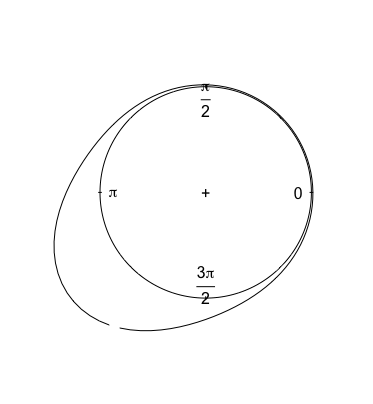
\includegraphics[clip,height= 40mm]{data/sample_symmetry.png}
  \end{center}
 \end{minipage}
\hspace{-1.0cm}
 \begin{minipage}{0.33\hsize}
  \begin{center}
 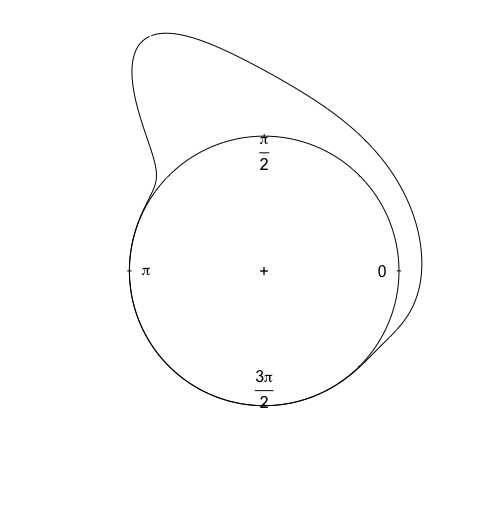
\includegraphics[clip,height= 40mm]{data/sample_asymmetry.png}
  \end{center}
 \end{minipage}
\hspace{-1.0cm}
 \begin{minipage}{0.33\hsize}
  \begin{center}
   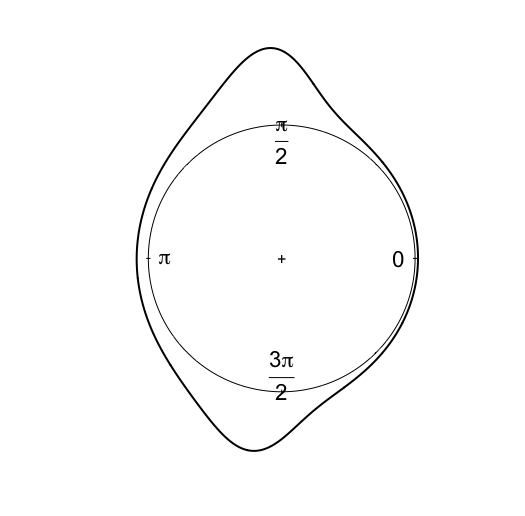
\includegraphics[clip,height= 40mm]{data/sample_bimodal.png}
  \end{center}
 \end{minipage}
  \end{tabular}
\caption[Text excluding the matrix]{
$\bm \mu = \begin{pmatrix} -1.2 \\ -0.95 \\ \end{pmatrix}, \Sigma = \begin{pmatrix}  1 & 0 \\ 0 & 1 \\ \end{pmatrix}$
とした場合の対称な射影正規分布(左), 
$\bm \mu = \begin{pmatrix} -0.19 \\ 2.09 \\ \end{pmatrix}, \Sigma = \begin{pmatrix} 2.49 & -1.85 \\ -1.85 & 1.96 \\ \end{pmatrix}$ とした場合の非対称な射影正規分布(中央), 
$\bm \mu = \begin{pmatrix} -0.24 \\ 0.15 \\ \end{pmatrix}, \Sigma = \begin{pmatrix}  0.209 & 0.068\\ 0.068 & 2.25 \\ \end{pmatrix}$ とした場合の二峰性となる射影正規分布(右)}
\label{sample_pn}
\end{figure}

% Wang and Gelfand(2013) によると各パラメータの単一の影響は良く分かっていない. だから各パラメータを細かく説明するのは困難である. しかしこの分布の柔軟な特性は予測などにおいて便利である.

\vspace{-2zh}
\subsection{混合射影正規分布}

$m$個のユニットからなる 射影正規分布の混合分布は以下のように定式化できる. 

\vspace{-2zh}
\begin{eqnarray*}
p(\theta;\bm w,\bm \mu, \Sigma) = \sum^m_{j=1} w_j \mathcal{PN}_2(\theta;\bm \mu_j, \Sigma_j) 
\end{eqnarray*}

\vspace{-1zh}
\noindent
ただし, $w_j$は混合比率であり, $0 < w_j < 1$, $\sum^m_{j=1} w_j = 1$を満たす. 混合射影正規分布におけるパラメータは, $w, \bm \mu_j, \Sigma_j$であるが, パラメータに識別可能性を保持するという制約を加えると共分散行列 $\Sigma$は

\vspace{-1zh}
\[
 \Sigma_j = \left(
    \begin{array}{cc}
      \tau_j^2 & \rho_j \tau_j \\
      \rho_j \tau_j & 1
    \end{array}
  \right)
\]

\vspace{-0.5zh}
\noindent
と定義されるので, パラメータベクトルは$\bm \eta = (w_1, \dots, w_m, \bm \mu_1, \dots, \bm \mu_m, \tau_1, \dots, \tau_m, \rho_1, \dots, \rho_m)^T$, パラメータベクトルの次元は $d = 4m$ となる. 各パラメータの事前分布を $\bm \mu_j \sim N(\bm 0, 10^5 \bm I_2)$, $\tau_j \sim \mathrm{half Cauchy}(0,5)$, $\rho_j \sim U(-1,1)$, $\bm w \sim Dirichlet(2,2, \dots, 2)$ と設定する. ここで混合比率$\bm w$は$m$次の$Dirichlet$分布に従うものとする. $\bm \mu_j$は$0$付近に存在するという背景を元に, 正規分布による弱情報事前分布とし, $\tau_j$は非負かつ値が大きくなりすぎないように, 裾の重いコーシー分布を$0$で切断した, 半コーシー分布を弱情報事前分布とする. $\rho_j$は$-1 \sim 1$に存在することが分かっているので, 一様分布を弱情報事前分布とし, $\bm w$は非負かつ和が $1$となる性質をもつディリクレ分布を弱情報事前分布とする.

角度データ $\theta$ が得られたときの, パラメータベクトル $\bm \eta$の事後分布を $p(\bm \eta| \theta)$, パラメータベクトルの事前分布を $p(\bm \eta)$とすると事後分布は以下で定義できる. 

\vspace{-1zh}
\begin{eqnarray*}
p(\bm \eta | \theta) = \frac{p(\theta | \bm \eta) p(\bm \eta)}{p(\theta)} \propto p(\theta | \bm \eta) p(\bm \eta)
\end{eqnarray*}

\vspace{-0.5zh}
\noindent
すなわち, 事後分布$p(\bm \eta | \theta)$は尤度$p(\theta | \bm \eta)$と事前分布 $p(\bm \eta| \theta)$の積に比例する. ここで, $p(\theta)$はすでに得られた, データ$\theta$にのみ依存する定数値であるので, $p(\theta | \bm \eta) p(\bm \eta)$が $\bm \eta$ の分布の形を作り, $p(\theta)$は正規化定数とみなすことができる. 尤度と事前分布の計算は簡単だが, 周辺分布 $p(\theta)$の計算は一般に簡単ではないので, 事後分布に比例する分布 $p(\theta | \bm \eta) p(\bm \eta)$ から乱数サンプルを発生させて事後分布の代わりとする. この方法で得られたサンプルをMCMCサンプルと呼ぶ. 尤度関数を式$\ref{logPN}$ に示す. 

\vspace{-2zh}
\begin{eqnarray}
\label{logPN}
\log p(\theta | \bm \eta) &=& \sum^m_{j=1} \{\log w_j + \log \mathcal{PN}_2(\theta;\bm \mu_j, \Sigma_j)\} \nonumber \\ 
&=& \sum^m_{j=1} \left[ \log w_j - \log 2\pi - \log A - \frac{1}{2} \log |\Sigma| + C + \log \left\{1 + \frac{B(\theta)}{\sqrt{A(\theta)}} \frac{\Phi \left(\frac{B(\theta)}{\sqrt{A(\theta)}}\right)}{\phi \left(\frac{B(\theta)}{\sqrt{A(\theta)}}\right)}\right\} \right] \nonumber \\
&\propto& \sum^m_{j=1} \left[ \log w_j - \log A - \frac{1}{2} \log |\Sigma| + C + \log \left\{1 + \frac{B(\theta)}{\sqrt{A(\theta)}} \frac{\Phi \left(\frac{B(\theta)}{\sqrt{A(\theta)}}\right)}{\phi \left(\frac{B(\theta)}{\sqrt{A(\theta)}}\right)}\right\} \right]  
\end{eqnarray}

%%%%%%%%%%%%%%%%%%%%%%%%%%%%%%%%%%%%%%%%%%%%%%%%%%%%%%%%%%%%%%%%%%%
%%%%%%%%%%%%%%%%%%%%%%%  sectio3 解析手法 %%%%%%%%%%%%%%%%%%%%%%%%

\section{解析手法}

\vspace{-0.5zh}
\subsection{マルコフ連鎖モンテカルロ法}

本研究ではMCMCアルゴリズムの一つである, ハミルトニアン$\cdot$モンテカルロ法(HMC)を用いて分布の推定を行う. HMCのアルゴリズムはハミルトン方程式の数学的性質によって正当性が保証されている. 一般の確率分布からのサンプリングについて, ハミルトン方程式を定義するには, 元の問題に存在しない仮想的な運動量を補助変数として導入する必要がある. 

HMCは物理学の考えを用いて, メトロポリスアルゴリズムによるランダムウォークな振る舞いを局所的に抑圧する. 従って, 目標の分布までより素早く推移することを可能にする. 対象となる確率変数 $(\bm \eta)$に対して, 速度変数$\bm \phi$を付与する. このメトロポリスアルゴリズムでは$\bm \eta, \bm \phi$を共に更新する. $\bm \eta$の各分布の推移には$\bm \phi$が大きく影響する. 

HMCでは, 事後確率 $p(\bm \eta| \theta)$ は$p(\bm \phi)$の独立な分布によって増大する. したがって結合分布を以下のように定義する.

\vspace{-1zh}
\begin{eqnarray*}
p(\bm \eta, \bm \phi| \theta) = p(\bm \phi) p(\bm \eta| \theta)
\end{eqnarray*}

$\bm \eta$をシュミレーションするために, 上記の結合分布によりパラメータをシュミレーションする. この補助変数$\bm \phi$を導入することでパラメータ空間をより効率的に移動することを可能にする. HMCは対数事後密度の勾配を要求する. $d$次元のパラメータ$\bm \eta$の勾配は以下で表す.

\vspace{-1zh}
\begin{eqnarray*}
\frac{d \log p(\bm \eta| \theta)}{d \bm \eta} = \left( 
  \frac{d \log p(\bm \eta| \theta)}{d \eta_1}, \dots,
  \frac{d \log p(\bm \eta| \theta)}{d \eta_d} \right)
\end{eqnarray*}

$\bm \phi$の事前分布については, 平均$0$, 共分散行列$M$の多変量正規分布を与える. $\bm \phi$の要素が独立の場合は各次元ごとに$\phi_j \sim N(0,M_{jj})$を与える. $M$は事後分布の逆共分散行列 $\Bigl(\mbox{var}(\bm \eta| \theta)\Bigr)^{-1}$で大まかにスケールすることができる. アルゴリズムはどんな場合でも動作するが, $M$のスケーリングが優れていることにより, HMCがより効率的となる.

HMCでは次の反復計算により事後分布からサンプリングを行う. 

\begin{enumerate}

\item{}
各速度変数 $\bm \phi$ を $\bm \phi \sim N(0,M)$からランダムサンプリングする.

\item{}
$\bm \eta, \bm \phi$を同時に更新する.

\vspace{-1zh}
\begin{eqnarray*}
\bm \phi_{t+\frac{1}{2}} \leftarrow \bm \phi_t + \frac{1}{2} \epsilon \frac{d \log p(\bm \eta| \theta)}{d \bm \eta}, 
\bm \eta_{t+1} \leftarrow \bm \eta_t + \epsilon M^{-1} \bm \phi_{t+\frac{1}{2}},
\bm \phi_{t+1} \leftarrow \bm \phi_{t+\frac{1}{2}} + \frac{1}{2} \epsilon \frac{d \log p(\bm \eta| \theta)}{d \eta_{t+1}}. 
\end{eqnarray*}

\item{}
得られたパラメータの採択, 棄却を決定する. 上記のステップで得られたパラメータを$\bm \eta^*, \bm \phi^*$として,
現在が$t$回目の反復とすると, サンプルの棄却率は

\vspace{-1zh}
$$ r = \frac{p(\eta \eta^*|y) p(\bm \phi^*)}{p(\bm \eta^{t-1}|y) p(\phi^{t-1})}$$

と定義され, $0$から$1$の間でランダムに選んだ数値より, $r$が高ければ$\bm \eta^*$を採択する. サンプル数が定めた値に達したら, 終了する.

\end{enumerate}

%%%%%%%%%%%%%%%%%%%%%%%%%%%%%%%%%%%%%%%%%%%%%%%%%%%%%%%%%%%%%%%%%%%
%%%%%%%%%%%%%%%%%%%%%%%  sectio4 数値実験 %%%%%%%%%%%%%%%%%%%%%%%%

\section{シミュレーション}

人工的データを用いて, 混合 Projected Normal 分布によるクラスタリングの性能評価を行う. 複数の von Mises 分布に従う乱数を発生させて, 1つのデータにまとめることで混合データを作成する. 

\subsection{解析データ}

$\mu(0 < \mu < 2\pi), \kappa(\kappa \geq 0) $をパラメータ, $\theta(0 \leq \theta < 2\pi)$を確率変数とする, Von Mises 分布の確率密度関数は以下の式で表せる. また式中の第一種変形ベッセル関数の定義式を示す.

\vspace{-1zh}
\begin{eqnarray*}
f(\theta;\mu, \kappa) = \frac{\exp[\kappa \cos(\theta - \mu)]}{2 \pi I_0(\kappa)} , I_j(\kappa) = \left(\frac{\kappa}{2}\right)^j \sum^\infty_{i=0} \frac{\left(\frac{\kappa^2}{4}\right)^i}{i \Gamma(j + i + 1)}
\end{eqnarray*}

ユニット数$m=4$, 角度$\theta = \left( \frac{7\pi}{4}, \frac{2\pi}{3}, \frac{5\pi}{4}, \frac{\pi}{6}\right)$, パラメータ$\kappa= (2,10,5,15)$, 混合比率$(0.4, 0.2, 0.3, 0.1)$として, 乱数を生成する. 

\vspace{-1zh}
\begin{figure}[H]
\begin{center}
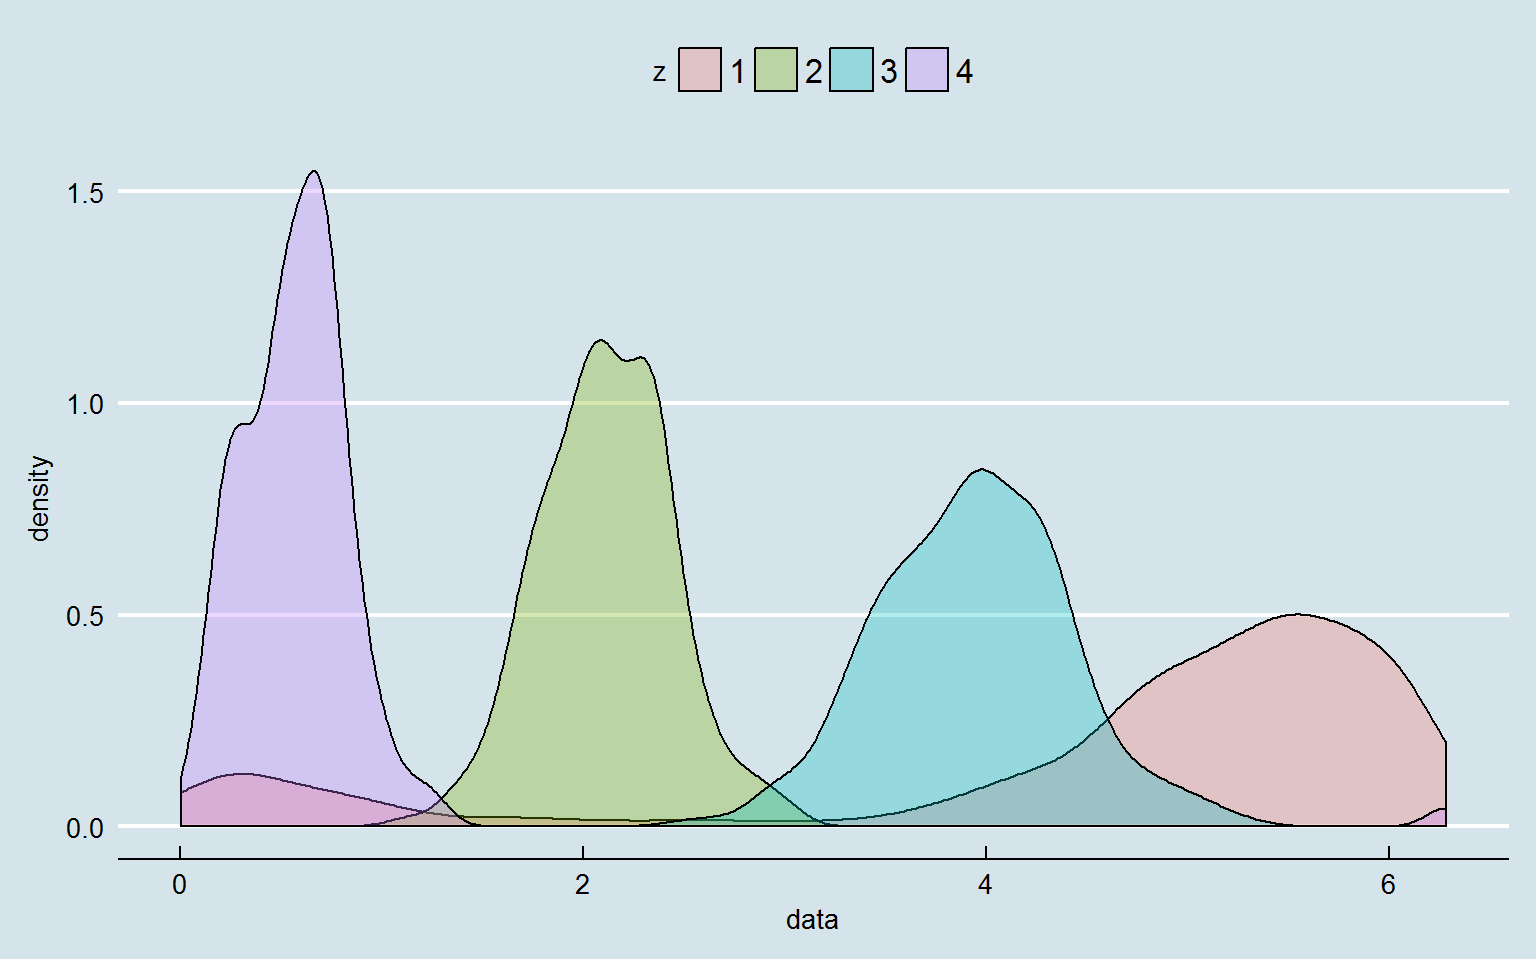
\includegraphics[clip,height= 35mm]{data/mix_test_data.png}
\end{center}
\caption{混合データ(クラスター数:4)}

\label{mixdata}
\end{figure}

\subsection{解析結果}

Mixture von Mises 分布では元のデータと同じく4つの元となる分布を推定したが, Mixture Projected Normal 分布においては3つの元となる分布により以下の結果が得られた.

\begin{figure}[h]
 \begin{tabular}{c}
\hspace{0.5cm}
 \begin{minipage}{0.5\hsize}
  \begin{center}
   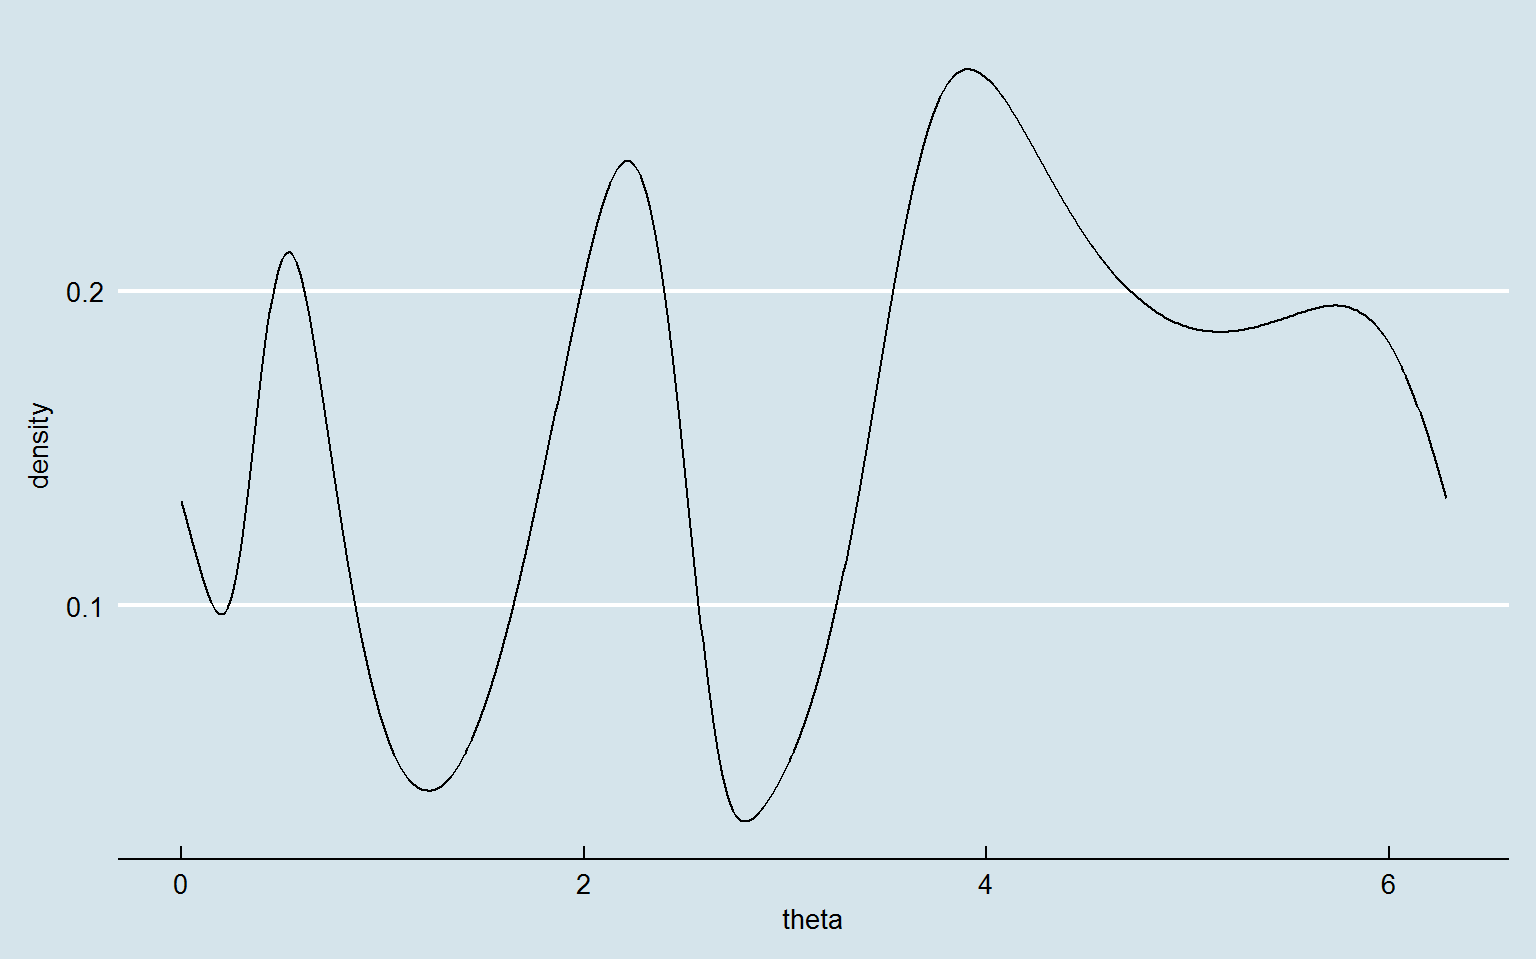
\includegraphics[clip,height= 35mm]{data/mix_pn.png}
  \end{center}
  %\caption{Mixture Projected Normal 分布により推定した混合分布}
  \label{pnmix}
 \end{minipage}
\hspace{-1.0cm}
 \begin{minipage}{0.5\hsize}
  \begin{center}
   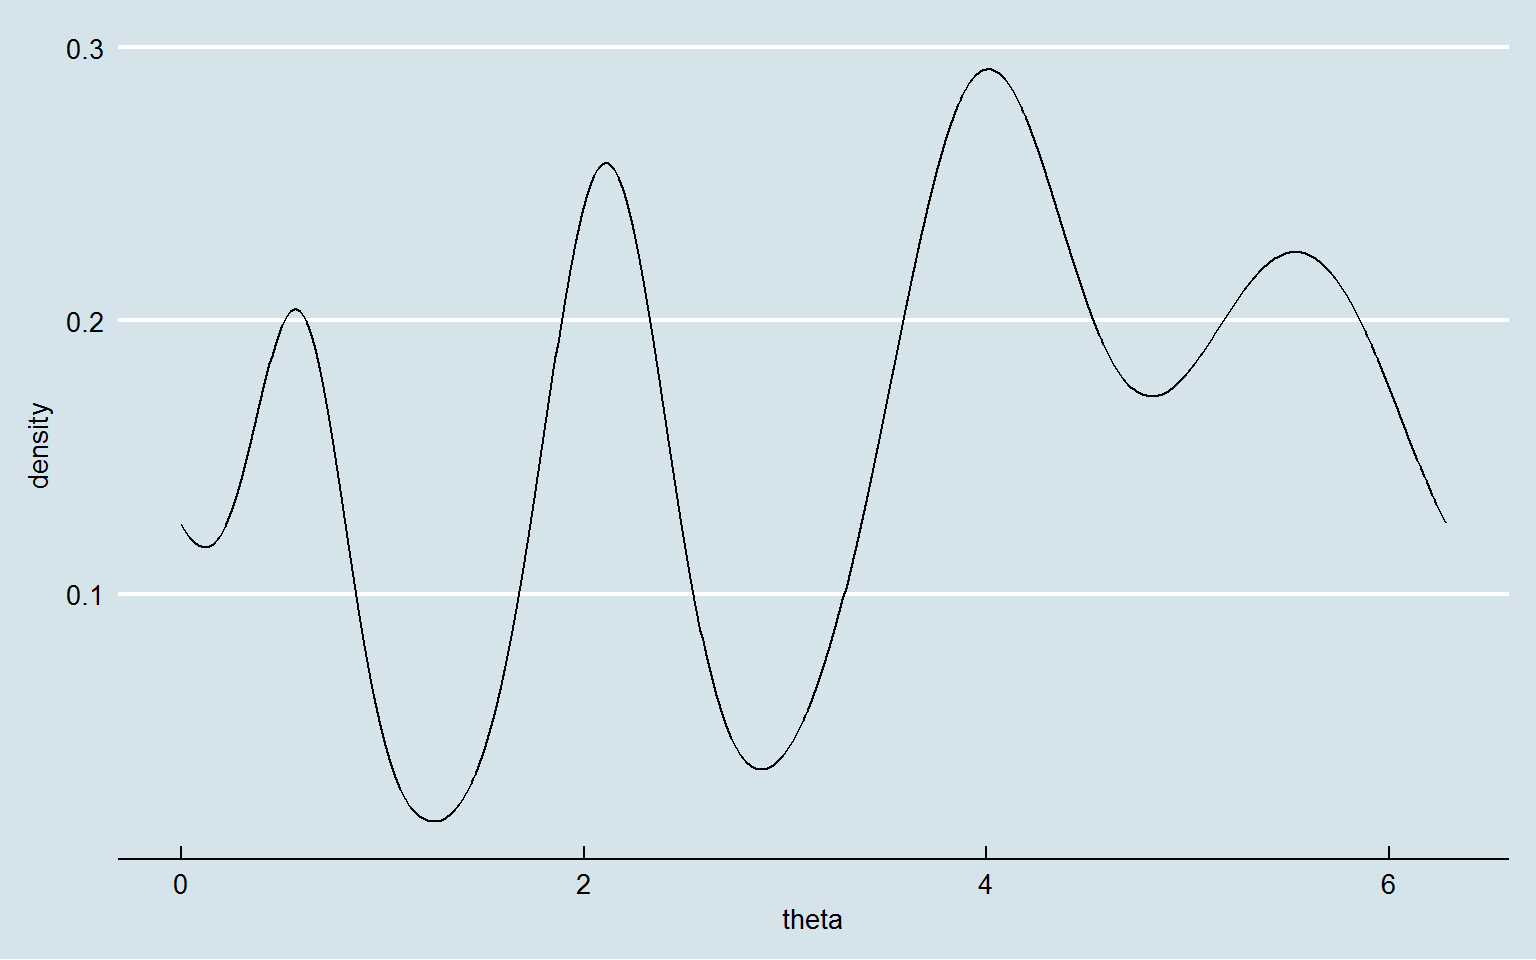
\includegraphics[clip,height= 35mm]{data/mix_von.png}
  \end{center}
 % \caption{Mixture von Mises分布により推定した混合分布}
  \label{vonmix}
 \end{minipage}
  \end{tabular}
\caption{Mixture Projected Normal 分布により推定した混合分布(左), Mixture von Mises分布により推定した混合分布(右)}
\end{figure}


得られた混合分布から, 混合データの分類を行う. 混合分布を構成する, 分布の中で出現確率が最も高いものをそのデータの予測クラスタとする.
横軸を真のクラスタ, 縦軸を予測クラスタとして集計表を示す. 

\begin{table}[H]
\caption{PN 分布によるクラスター推定(左), VM 分布によるクラスター推定(右)}
\begin{tabular}{c}
% 1
\hspace{1.5cm}
\begin{minipage}{0.5\hsize}
\begin{center}
%\caption{PN 分布によるクラスター推定}
\begin{tabular}{|c|c|c|c|c|}
\hline
 &  & \multicolumn{3}{|c|}{Predict} \\ \hline
 &  & 1 & 2 & 3 \\ \hline 
 &1 & 38 & 10 & 352 \\ \cline{2-5}
True
 & 2 & 1 & 192 & 7 \\ \cline{2-5}
 & 3 & 0 & 2  & 298 \\ \cline{2-5}
 & 4 & 93 & 0 & 7 \\ 
\hline
 \end{tabular}
 \end{center}
\end{minipage}

% 2
\hspace{-2.5cm}
\begin{minipage}{0.5\hsize}
\begin{center}
%\caption{VM 分布によるクラスター推定}
\begin{tabular}{|c|c|c|c|c|c|}
\hline
 &  & \multicolumn{4}{|c|}{Predict} \\ \hline
 &  & 1 & 2 & 3 & 4 \\ \hline 
 & 1 & 333 & 10 & 39 & 18 \\ \cline{2-6}
True
 & 2 & 7 & 192 & 1 & 0 \\ \cline{2-6}
 & 3 & 298 & 2  & 0 & 0 \\ \cline{2-6}
 & 4 & 0 & 1 & 94 & 5 \\ 
\hline
\end{tabular}
\end{center}
\end{minipage}

\end{tabular}
\end{table}

%%%%%%%%%%%%%%%%%%%%%%%%%%%%%%%%%%%%%%%%%%%%%%%%%%%%%%%%%%%%%%%%%%%%%%
%%%%%%%%%%%%%%%%%%%%%%%  section5 まとめ %%%%%%%%%%%%%%%%%%%%%%%%%%%%%

\section{まとめ}

現在超球面上のクラスタリングは, テキストマイニングなどの分野に用いられている. 本研究で作成した混合 Projected Normal 分布をテキストマイニングに適用する.

%\newpage
\addcontentsline{toc}{section}{参考文献} %目次に参考文献を入れる

%必要になる
%\newpage
%\section{付録}

%参考文献を引用する際に必要なコマンド
\bibliographystyle{jplain}
\bibliography{bunken}

%%%%%%%%%%%%%%%%%%%%%%%%%%%%%%%%%%%%%%%%%%%%%%%%%%%%%%%%%%%%%%%%%%%
%%%%%%%%% 参考文献用 bibtexから呼び出すページ %%%%%%%%%%%%%%%%%%%%%%%%%%

\newpage

関係ないページです!

Presnell(1998) \cite{PML}

Wang and Gelfand (2013) \cite{PN1}

D. Hemandez(2017) \cite{GPN}

Dhillon and Modha(2001) \cite{SKMcluster}

Gopal and Yang(2014) \cite{Gopal}

\if0
%%%%%%%% 図の挿入用 %%%%%%%%%%%%%%
\vspace{-0.3cm}
\begin{figure}[H]
\begin{center}
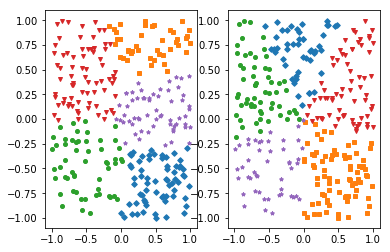
\includegraphics[clip,height= 35mm]{data/kmeans+skmeans.png}
\end{center}
 \vspace{-0.9cm}
\caption{k-meansによるクラスタリング(左), skmeansによるクラスタリング(右)}
\label{skmeans}
\end{figure}

%%%%%%%% 回り込み図の挿入用 %%%%%%%%%%%%%%
\begin{wrapfigure}[10]{r}[5mm]{70mm}
\vspace{-0.6cm}
\centering
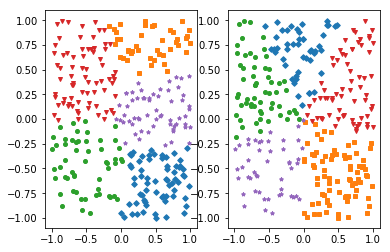
\includegraphics[keepaspectratio,width=70mm]{data/kmeans+skmeans.png}
\vspace{-1cm}
\caption{k-meansによるクラスタリング(左), skmeansによるクラスタリング(右)}
\label{kmeans}
\end{wrapfigure}
\fi

\end{document}

%\begin{table}[H]
%\begin{center}
%\caption{条件付確率表(CPT)}   %キャプション
%\label{cpt}   %ラベル
%\begin{tabular}{|c||c|c|c|}   %{}で文字の揃え方を指定
%\hline
% & $Pa(X_{j})=x_{1}$ & \dots & $Pa(X_{j})=x_{m}$
%\\ \hline
%$X_j=y_1$ & $p(y_1|Pa(X_j)=x_1)$ & \dots & $p(y_1|Pa(X_j)=x_m)$
%\\ \hline
%$\vdots$ & $\vdots$ & $\ddots$ & $\vdots$
%\\ \hline
%$X_j=y_n$ & $ p(y_n|Pa(X_j)=x_1)$ & \dots & $p(y_n|Pa(X_j)=x_m)$
%\\ \hline
%\end{tabular}
%\end{center}
%\end{table}
